\documentclass[conference]{IEEEtran}
\IEEEoverridecommandlockouts
\usepackage{cite}
\usepackage{amsmath,amssymb}
\usepackage{graphicx}
\usepackage{booktabs}
\usepackage{url}
\usepackage{balance}          % even out the two columns on the final page
\usepackage[hidelinks]{hyperref}

\newcommand{\px}{\,px}
\newcommand{\ms}{\,ms}

\begin{document}

\title{NeuFlow v3: Queryable Optical Flow with\\ Calibrated Uncertainty for
Region-Directed Perception}

\author{\IEEEauthorblockN{Shriman Raghav Srinivasan}
\IEEEauthorblockA{\textit{Department of Electrical and Computer Engineering} \\
\textit{Northeastern University}\\
Boston, MA, USA}}

\maketitle

\begin{abstract}
Optical flow networks emit a dense displacement field at a single fixed
resolution. Many consumers of flow, including image registration, sparse
tracking and survey mosaicking, require a few hundred correspondences at
locations they select rather than a value at every pixel. We present NeuFlow v3,
which retains the NeuFlow v2 pipeline through its coarse flow stage and replaces
only the final convex upsampler with an implicit decoder evaluated at arbitrary
continuous coordinates. We pursue three objectives: queryable output, so cost
scales with the number of queries, $O(N)$, rather than with image area,
$O(H{\times}W)$; cheap repeatability, so a frame pair is processed once and every
subsequent query is answered from cached state at 1.25\ms\ against 33.3\ms, a
factor of $27$; and calibrated confidence, a per-query error scale the baseline
cannot express at all. The decoder is 745{,}226 parameters, 38\% of the stage it
replaces, and the complete model is 13.3\% smaller than the baseline. On held-out
driving sequences it is 2.6\% less accurate on mean end-point error. The
confidence signal is the more consequential capability: ranking queries by
predicted error lets the model abstain on its least confident 20\%, reducing mean
error over the remaining 80\% of the frame to 1.06\px, a selection the baseline
cannot make at any threshold since it emits flow alone. We further
characterise region-directed inference for fast-moving platforms, showing that
the context margin a cropped region requires is set by inter-frame displacement
rather than image size, a relation we verify at two motion scales differing by a
factor of three.
\end{abstract}

\begin{IEEEkeywords}
optical flow, implicit neural representation, uncertainty estimation, edge
computing, region of interest
\end{IEEEkeywords}

\section{Introduction}

Optical flow estimation has converged on a common output contract: given two
frames, produce a displacement vector for every pixel, at the resolution of the
input. Modern real-time networks such as NeuFlow v2~\cite{neuflow2} attain this
efficiently enough for embedded deployment. The contract itself, however, is
rarely questioned, and it does not match what several important consumers of
flow actually require.

Image registration selects a few hundred well-textured points and needs
correspondences at those points. Sparse feature tracking needs flow at detected
keypoints. Survey mosaicking needs matches within overlap regions, frequently at
sub-pixel positions. In each case a dense field is computed, and the great
majority of it is discarded. On constrained hardware, computing 479{,}232
correspondences in order to consume 800 of them is the difference between
operating in real time and not.

The fixed-resolution contract also forecloses two operations outright. A
consumer cannot request flow at a position between input pixels, and it cannot
request additional correspondences on a frame the network has already processed
without paying for the entire computation again.

This paper asks whether the final stage of a real-time flow network can be made
queryable without surrendering accuracy or throughput, and reports what such a
change costs and what it buys. We pursue three objectives, each of which the
results section addresses in turn:

\begin{enumerate}
\item \textbf{Queryable output.} An implicit decoder replaces NeuFlow v2's convex
      upsampler and answers flow queries at arbitrary continuous coordinates in
      $O(N)$ rather than $O(H{\times}W)$, with sparse output identical to dense
      output at matching coordinates to 0.00057\px.
\item \textbf{Cheap repeatability.} The network is factored into a coarse pass
      computed once per frame pair and cached, and a decode evaluated against
      that cached state. A repeat query costs 1.25\ms\ against the baseline's
      33.3\ms\ full recomputation, a factor of $27$, because the baseline retains
      nothing between calls.
\item \textbf{Calibrated confidence.} A per-query error scale $b$ under a Laplace
      likelihood, monotonic over a $15\times$ range of predicted values, which
      enables selective prediction: $2.2\times$ lower error than the baseline
      over 80\% of the frame. The baseline emits flow alone and cannot abstain at
      any price.
\end{enumerate}

Two further results accompany them. We characterise region-directed inference for
fast platforms, including a design rule relating the required context margin to
platform speed and frame rate, verified across two domains whose motion scales
differ by a factor of three. And we account explicitly for what the change costs:
2.6\% of mean accuracy on the training domain, with the mechanism identified.

\begin{figure*}[t]
\centering
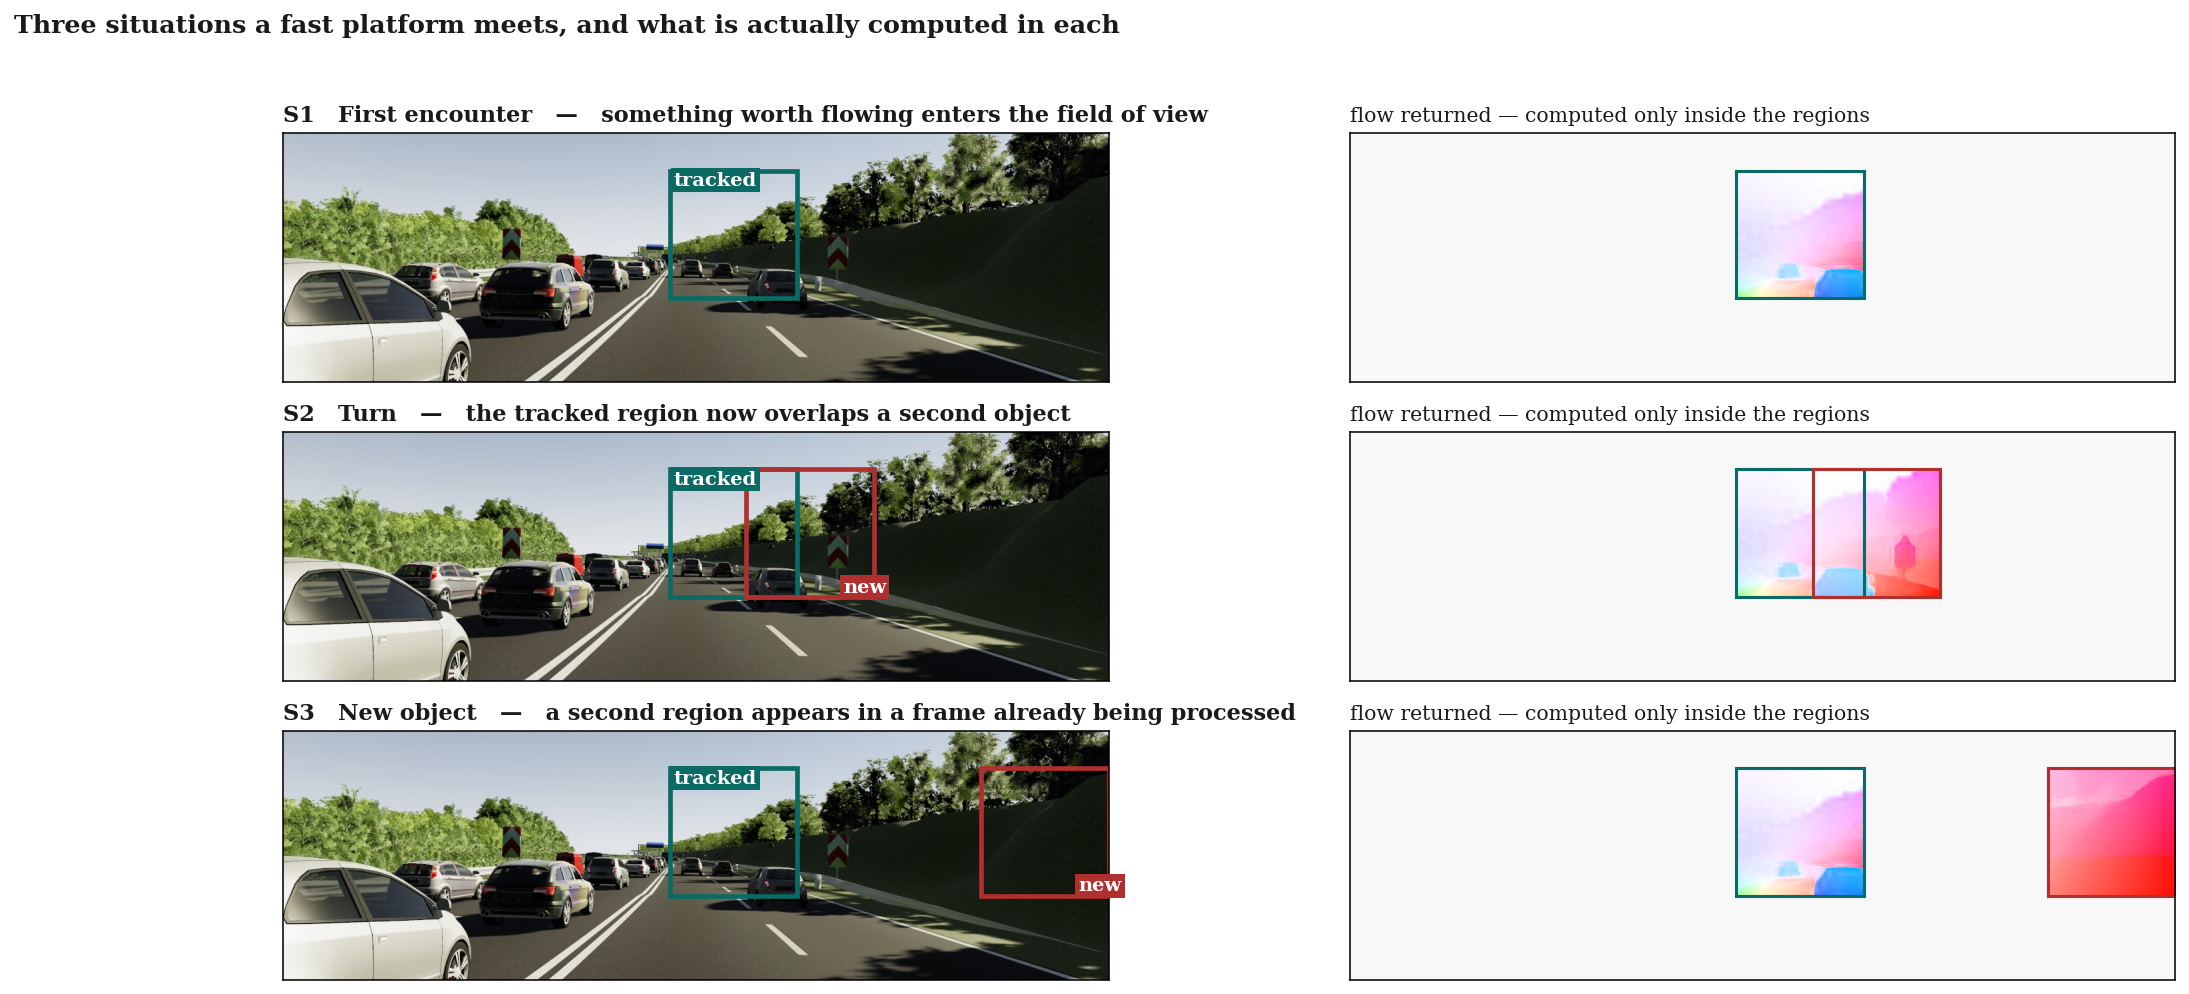
\includegraphics[width=\textwidth]{figures/scenarios_illustrated.png}
\caption{Three situations a fast platform encounters, on held-out driving
frames. Left: the frame with the region or regions a tracker would nominate.
Right: the flow the decoder actually returns, computed only inside those
regions. Top, a first encounter; middle, a turn in which the tracked region
comes to overlap a second object; bottom, a new object appearing in a frame
already being processed, which the decoder answers from cached state.}
\label{fig:scenarios}
\end{figure*}

\section{Related Work}

\textbf{Variational and local methods.} Horn and Schunck~\cite{hs81} pose flow as
the minimisation of a global energy pairing brightness constancy with a
smoothness penalty on the field. Lucas and Kanade~\cite{lk81} solve brightness
constancy in closed form over a window in which the flow is assumed constant.
Both are local by construction, because the data term is a first-order expansion
about zero displacement and holds only while motion is small relative to image
structure. Brox et al.~\cite{brox04} add gradient constancy and a coarse-to-fine
warping scheme, which extends the usable range but still loses a small object
that moves far enough to vanish from the coarsest level. Large displacement of
small structures is the failure every learned method since has been measured
against.

\textbf{Learned flow.} FlowNet~\cite{flownet} replaced the energy with a network
trained end to end on synthetic data, and showed that an explicit correlation
layer between the two frames helps more than letting a generic encoder discover
matching on its own. FlowNet 2.0~\cite{flownet2} closed the remaining gap to
variational accuracy by stacking several such networks with warping between them,
at the cost of a large model. PWC-Net~\cite{pwcnet} and
LiteFlowNet~\cite{liteflownet} put the classical pyramid back inside the network:
flow from the coarser level warps the second frame and a cost volume is built
over a bounded displacement range around that warp, which is what made these
models compact enough to be practical. The cascade's own weakness is that an
error made at a coarse level is never revisited. RAFT~\cite{raft} removed the
cascade by building one all-pairs correlation volume at $1/8$ resolution and
reading from it repeatedly with a recurrent unit, refining a single estimate at
fixed resolution; it set the accuracy standard the field still works against, at
considerable cost. GMFlow~\cite{gmflow} instead treats correspondence as global
matching, with cross-attention over the whole feature map producing flow directly
and refinement reduced to a correction.

\textbf{Real-time flow.} NeuFlow~\cite{neuflow1} keeps global matching but runs it
at $1/16$ behind a shallow backbone, then refines with cheap recurrent updates.
NeuFlow v2~\cite{neuflow2} restructures the backbone and refinement and ends with
a learned convex upsampler that predicts blending weights over a $3{\times}3$
neighbourhood of coarse flow. That upsampler is the stage we replace, and
everything above it we inherit frozen.

\textbf{Implicit representations.} NeRF~\cite{nerf} showed that a
coordinate-conditioned MLP can hold a scene and be evaluated anywhere in it, and
SIREN~\cite{siren} showed that the activation function bounds how much
high-frequency detail such a network can hold at all. LIIF~\cite{liif} made the
discrete-to-continuous step for images: a local latent code plus a relative
coordinate, decoded by one shared MLP, so a single trained model can be sampled
at any resolution. AnyFlow~\cite{anyflow} brought arbitrary-scale decoding to
flow by predicting convex weights over candidate displacements, which is the
formulation our head adopts. It is built on RAFT and reports no inference
timings, leaving open whether the approach survives a real-time budget.
InfiniDepth~\cite{infinidepth} does the continuous version for depth and
contributes the gated hierarchical fusion of multi-scale features that our
decoder uses.

\textbf{Uncertainty.} Kendall and Gal~\cite{kendall} separate aleatoric from
epistemic uncertainty and train a heteroscedastic likelihood whose predicted
scale is supervised only by the error it explains. Ilg et al.~\cite{ilg18}
applied this to flow directly, comparing multi-hypothesis networks against a
single predictive distribution and showing that the estimate is usable rather
than decorative. PDC-Net~\cite{pdcnet} predicts a mixture density per
correspondence and uses it to decide which matches to trust, which is the use we
make of our per-query scale. We differ in predicting the scale per query rather
than per pixel, so it is available for exactly the correspondences the consumer
selected, and we evaluate it by selective prediction rather than by correlation
alone.

\textbf{The gap.} Every method above emits a dense field at one fixed resolution,
chosen when the network is built. Those that are queryable are queryable in
scale, not in coordinate, and the implicit decoders that are queryable in
coordinate have not been placed inside a network operating under a millisecond
budget. Whether arbitrary-coordinate querying is affordable at speed is therefore
open. That is what this paper measures.

\section{Method}

\subsection{Inherited Pipeline}

NeuFlow v2 extracts features at $1/8$ and $1/16$ resolution with a shallow CNN,
applies cross-attention and global matching at $1/16$ to establish an initial
flow, refines it recurrently (one iteration at $1/16$, eight at $1/8$), and
upsamples the resulting $1/8$-resolution flow with a learned convex combination
over a $3{\times}3$ neighbourhood. That upsampling stage, comprising the
full-resolution stem that feeds it and the convolutions that predict a separate
nine-way softmax for each of the 64 sub-pixels in every $8{\times}8$ cell, is
1{,}947{,}968 parameters.

We retain everything through the coarse flow, with all learned weights and all
normalisation statistics frozen at their published values. We verify this per
checkpoint: all 137 tensors shared with the baseline are bit-identical, so the
comparisons that follow isolate the decoder.

\subsection{Implicit Decoder}

The decoder operates in two phases, which is what makes repeat queries cheap.

\textbf{Phase 1}, once per frame pair. The frozen pipeline produces the coarse
flow and feature maps, which are cached as state.

\textbf{Phase 2}, once per query batch. For a query coordinate $(x, y)$ the
decoder bilinearly samples $3{\times}3$ windows from four sources: $1/8$
context, $1/8$ matching features, $1/16$ features, and frame-1 features warped by
the coarse flow. These are fused by a gated hierarchical MLP following
InfiniDepth, and the result conditions a head predicting weights over ten
candidates: the nine coarse-flow values in the local neighbourhood, plus a
bilinear sample at the query position.

The output is a convex combination,
\begin{equation}
\mathbf{f}(x,y) = \sum_{i=1}^{10} w_i(x,y)\, \mathbf{c}_i(x,y),
\quad \sum_i w_i = 1,\ w_i \geq 0,
\end{equation}
where $\mathbf{c}_i$ are the candidate displacements and $w_i$ are softmax
weights. Boundedness matters: the prediction cannot leave the convex hull of
locally supported motion, so the decoder cannot hallucinate displacement its
inputs do not support.

We initialise the head so that the softmax concentrates on the bilinear
candidate. An untrained decoder is therefore equivalent to bilinear upsampling
(0.011\px\ maximum deviation), and training can only depart from that known-good
operating point by learning.

The decoder is 745{,}226 trainable parameters, 38\% of the 1{,}947{,}968-parameter
stage it replaces. The complete model is 7{,}826{,}794 parameters against the
baseline's 9{,}029{,}536, 13.3\% smaller.

\subsection{Uncertainty Head}

An optional eleventh output predicts a per-query error scale $b$, trained under a
Laplace likelihood jointly with the flow loss,
\begin{equation}
\mathcal{L}_u = \frac{|\mathbf{f} - \mathbf{f}^*|}{b} + 2 \log b .
\end{equation}
Predicting a large $b$ is therefore only worth it where the error really is
large. The head is 65 parameters, zero-initialised so that $b = 1\px$ before
training. It costs no measurable inference time and attaches a confidence value
to every returned correspondence.

\subsection{Interface}

The interface is two calls, Fig.~\ref{fig:api}: one coarse pass per frame pair,
then any number of decodes against the cached state. Coordinates are
continuous, so $(312.7, 188.2)$ is as valid an argument as $(312, 188)$.

\begin{figure}[t]
\begin{footnotesize}
\begin{verbatim}
st = model.infer_coarse_state(img0, img1)

# arbitrary coordinates
flow = model.decode_queries(st, query_coords=q)

# or any output resolution
flow = model.decode_queries(st, tgt_h, tgt_w)

# with per-query confidence
flow, b = model.decode_queries(st, q,
              return_uncertainty=True)
\end{verbatim}
\end{footnotesize}
\caption{The complete interface. The coarse state is computed once per frame
pair; each further decode reuses it.}
\label{fig:api}
\end{figure}

\section{Experimental Setup}

\textbf{Evaluation.} Virtual KITTI 2~\cite{vkitti2} Scenes 18 and 20:
1{,}174 frame pairs, 460{,}573{,}660 valid pixels, per-pixel metrics. Both scenes
are excluded from every training set, enforced in the data loader and verified at
pair and frame level before each run. Cross-domain evaluation uses
TartanAir~\cite{tartanair} aerial sequences, which no model in this study was
trained on.

\textbf{Training.} All runs are generated from a single template so that any two
differ in exactly one variable: seed 1234, batch size 16, learning rate
$2\times10^{-4}$ under a OneCycle schedule, loss weighting $\gamma = 0.8$,
4{,}096 supervision queries per image, refinement schedule matching the
evaluation configuration, 100{,}000 steps, backbone frozen throughout.

\textbf{Hardware.} NVIDIA RTX 4060 laptop GPU, fp16, $384{\times}1248$ input
unless stated. Where a figure is device-dependent we report each device
separately.

\section{Results}

The three subsections that follow address the three objectives in order, after
which we account for what they cost and characterise region-directed inference.

\subsection{Objective 1: Queryable Output}

\begin{figure}[t]
\centering
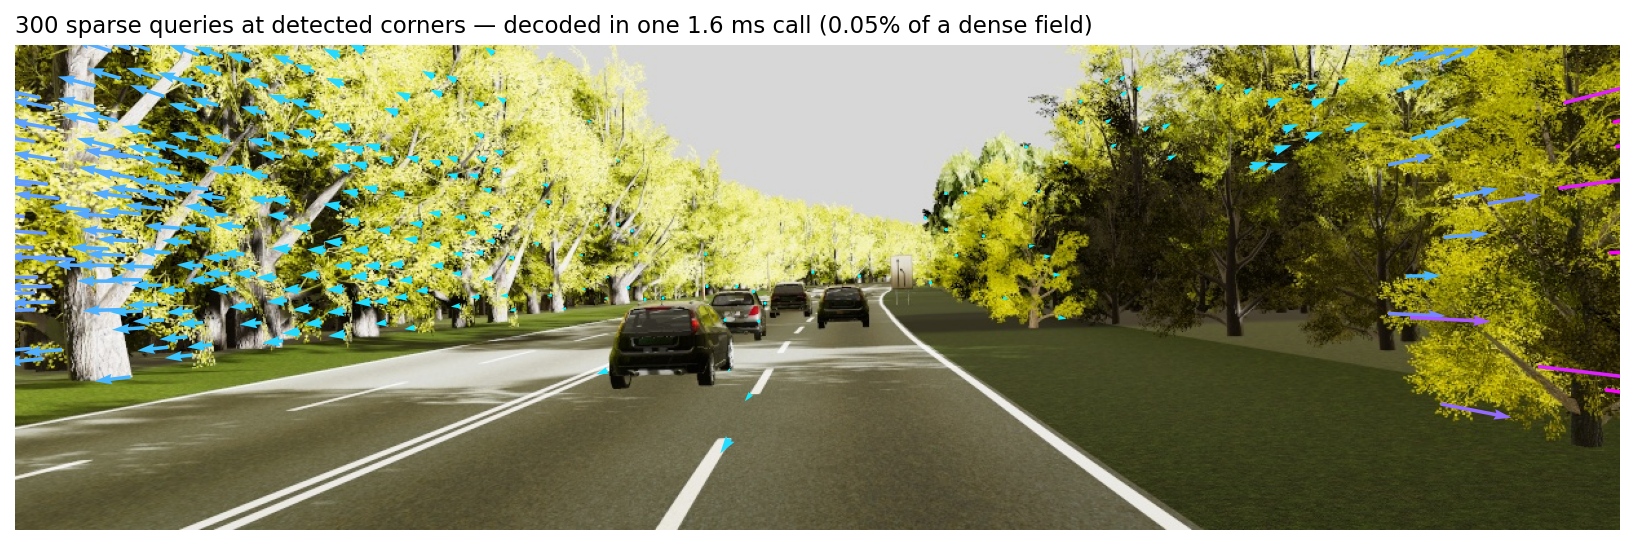
\includegraphics[width=\columnwidth]{figures/sparse_queries.png}
\caption{300 queries at detected corners, decoded in one call: 0.05\% of the
points a dense field would compute. Producing the same 300 answers from the
baseline means computing 479{,}232 and discarding 478{,}932 of them.}
\label{fig:sparse}
\end{figure}

The decoder takes a batch of continuous coordinates and returns flow at those
coordinates and nowhere else (Fig.~\ref{fig:sparse}). A corner detector selects
its own points, they enter one decode call, and cost scales with how many were
asked for.

Sparse and dense are not two modes but one function evaluated at different point
sets: sparse output reproduces the dense field to 0.00057\px\ maximum deviation
at matching coordinates, which we verify before every run. Decode latency is flat
in the query count over the operating range, 1.254\ms\ at $N{=}800$ and 1.285\ms\
at $N{=}2{,}048$, being bounded by kernel launch overhead rather than arithmetic,
so 2{,}048 points cost what 800 do.

\subsection{Objective 2: Cheap Repeatability}

\begin{table}[t]
\caption{Latency per frame pair}
\label{tab:speed}
\centering
\begin{tabular}{lrl}
\toprule
Mode & Latency & Note \\
\midrule
v2, full frame & 33.3\ms & its only mode \\
v3, first sparse query & 34.1\ms & level with v2 \\
\textbf{v3, repeat query} & \textbf{1.25\ms} & \textbf{$27\times$ cheaper} \\
v3, dense output & 37.1\ms & not the intended mode \\
\bottomrule
\end{tabular}
\end{table}

The sparse path comprises a 32.8\ms\ coarse pass, inherited unchanged, and a
1.25\ms\ decode. Because global matching requires whole-image context, the coarse
pass cannot be avoided; it accounts for 96\% of a first query, which is why a
first query costs what a baseline frame costs. We do not claim an advantage
there.

The decisive property is state reuse. The baseline retains nothing between
calls, so a second question about the same frame pair requires recomputing
everything: 33.3\ms\ against 1.25\ms, a factor of 27. Three questions about one
frame pair therefore cost the baseline 99.9\ms. The difference is structural
rather than an optimisation gap, and it is what the two-phase factorisation
exists to produce. In dense output mode, where nothing is reused, the baseline is
the faster of the two at 33.3\ms\ against 37.1\ms.

\subsection{Objective 3: Calibrated Confidence}

\begin{table}[t]
\caption{Error of the accepted set at each coverage level}
\label{tab:sel}
\centering
\begin{tabular}{lrr}
\toprule
Coverage & NeuFlow v3 & NeuFlow v2 \\
\midrule
20\% & \textbf{0.480} & 2.324 \\
40\% & 0.688 & 2.324 \\
60\% & 0.798 & 2.324 \\
80\% & \textbf{1.058} & 2.324 \\
100\% & 2.266 & 2.324 \\
\bottomrule
\end{tabular}
\end{table}

\begin{figure}[t]
\centering
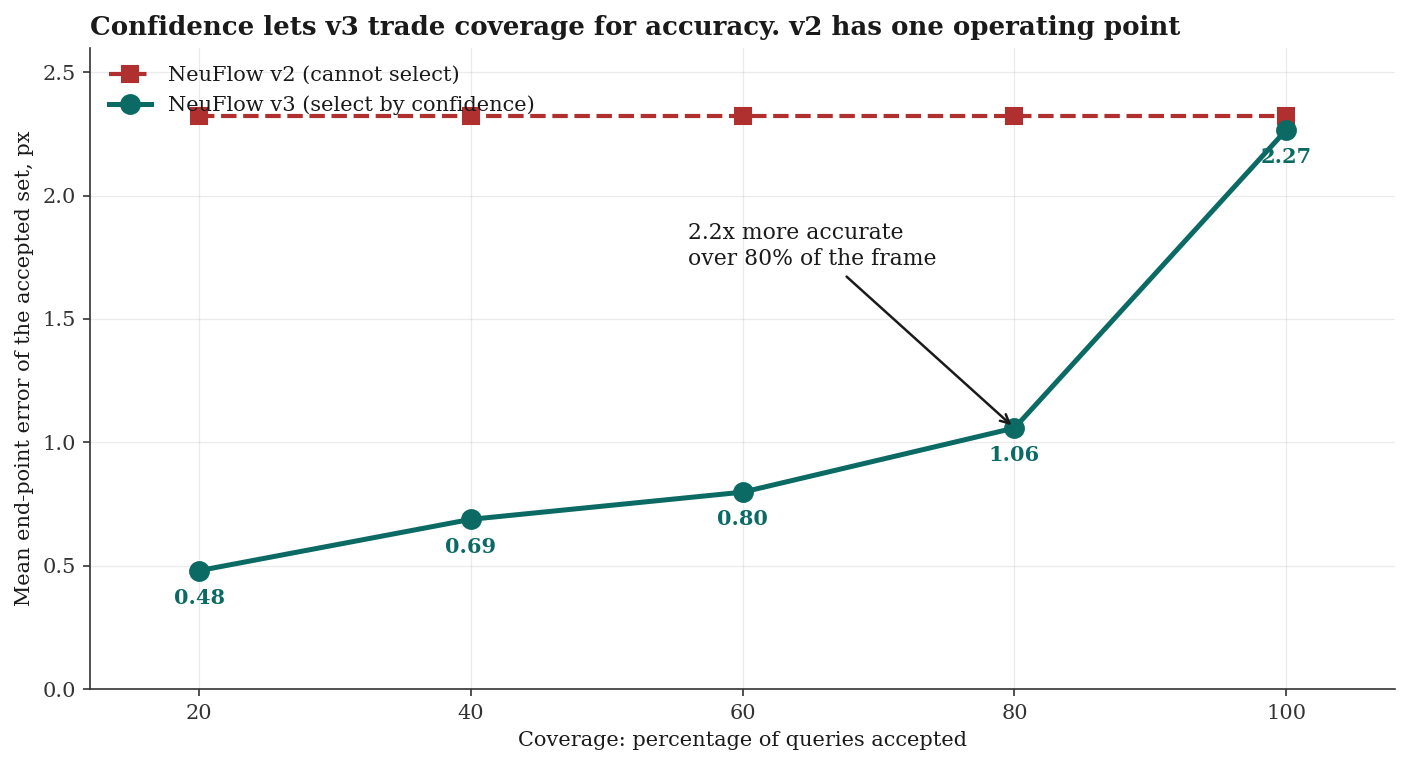
\includegraphics[width=\columnwidth]{figures/selective_accuracy.png}
\caption{Risk-coverage behaviour. The baseline has one operating point because
it cannot indicate which outputs to trust; per-query confidence gives the
decoder a curve.}
\label{fig:selective}
\end{figure}

Over 2{,}348{,}000 queries, actual error rises monotonically with predicted scale
across all five equal-count bins, from 0.480\px\ in the most confident to
7.100\px\ in the least, a factor of 15, with Pearson correlation 0.318. The
correlation is informative rather than tight, and we do not claim otherwise; what
a consumer uses is the ordering, and the ordering is correct.

Mean error over every pixel is a single operating point, and it is the only one
the baseline has, because it cannot indicate which of its outputs to trust. Given
a per-query confidence, v3 has a curve (Table~\ref{tab:sel},
Fig.~\ref{fig:selective}). Discarding the least confident 20\% of queries reduces
error on the remainder to 1.058\px\ against the baseline's 2.324\px, more than
twice as accurate over 80\% of the frame. Retaining only the most confident fifth
gives 0.480\px.

The obvious objection is that the accepted 80\% may simply be the easier 80\%. We
therefore scored both models on an identical query set, the matched subset the
decoder accepts, and the result holds. Beyond that comparison the point is a
capability rather than a margin: the baseline has no mechanism for selecting
among its own outputs, so it cannot trade coverage for accuracy at any price.

\subsection{The Cost in Accuracy}

\begin{table}[t]
\caption{Accuracy on held-out driving sequences}
\label{tab:acc}
\centering
\begin{tabular}{llrrr}
\toprule
Model & Training data & EPE & 1px & 3px \\
\midrule
NeuFlow v2 & FlyingThings & \textbf{2.324} & \textbf{77.6} & \textbf{89.8} \\
NeuFlow v3 & FlyingChairs & 2.500 & 72.8 & 87.9 \\
NeuFlow v3 & \; + VKITTI2 & 2.398 & 75.7 & 88.9 \\
NeuFlow v3 & \; + Sintel & 2.392 & 75.8 & 89.0 \\
NeuFlow v3 & \; + uncertainty & 2.384 & 76.1 & 89.0 \\
\bottomrule
\end{tabular}
\end{table}

Table~\ref{tab:acc} reports what the three objectives cost. Every v3
configuration is less accurate than the baseline. The best is 2.6\% worse on mean
end-point error and 1.5 points worse on 1-pixel accuracy; the like-for-like
comparison, trained on FlyingChairs alone as the baseline was trained on
FlyingThings alone, is 7.6\% behind. The cost is paid once, by a decoder that is
38\% of the size of the stage it replaces, in a model 13.3\% smaller overall.

The ordering across training mixes is monotonic, though the last three
configurations differ by less than 0.02\px\ and we do not draw conclusions from
their ranking under a single seed.

\subsection{Cross-Domain Comparison}

\begin{figure*}[t]
\centering
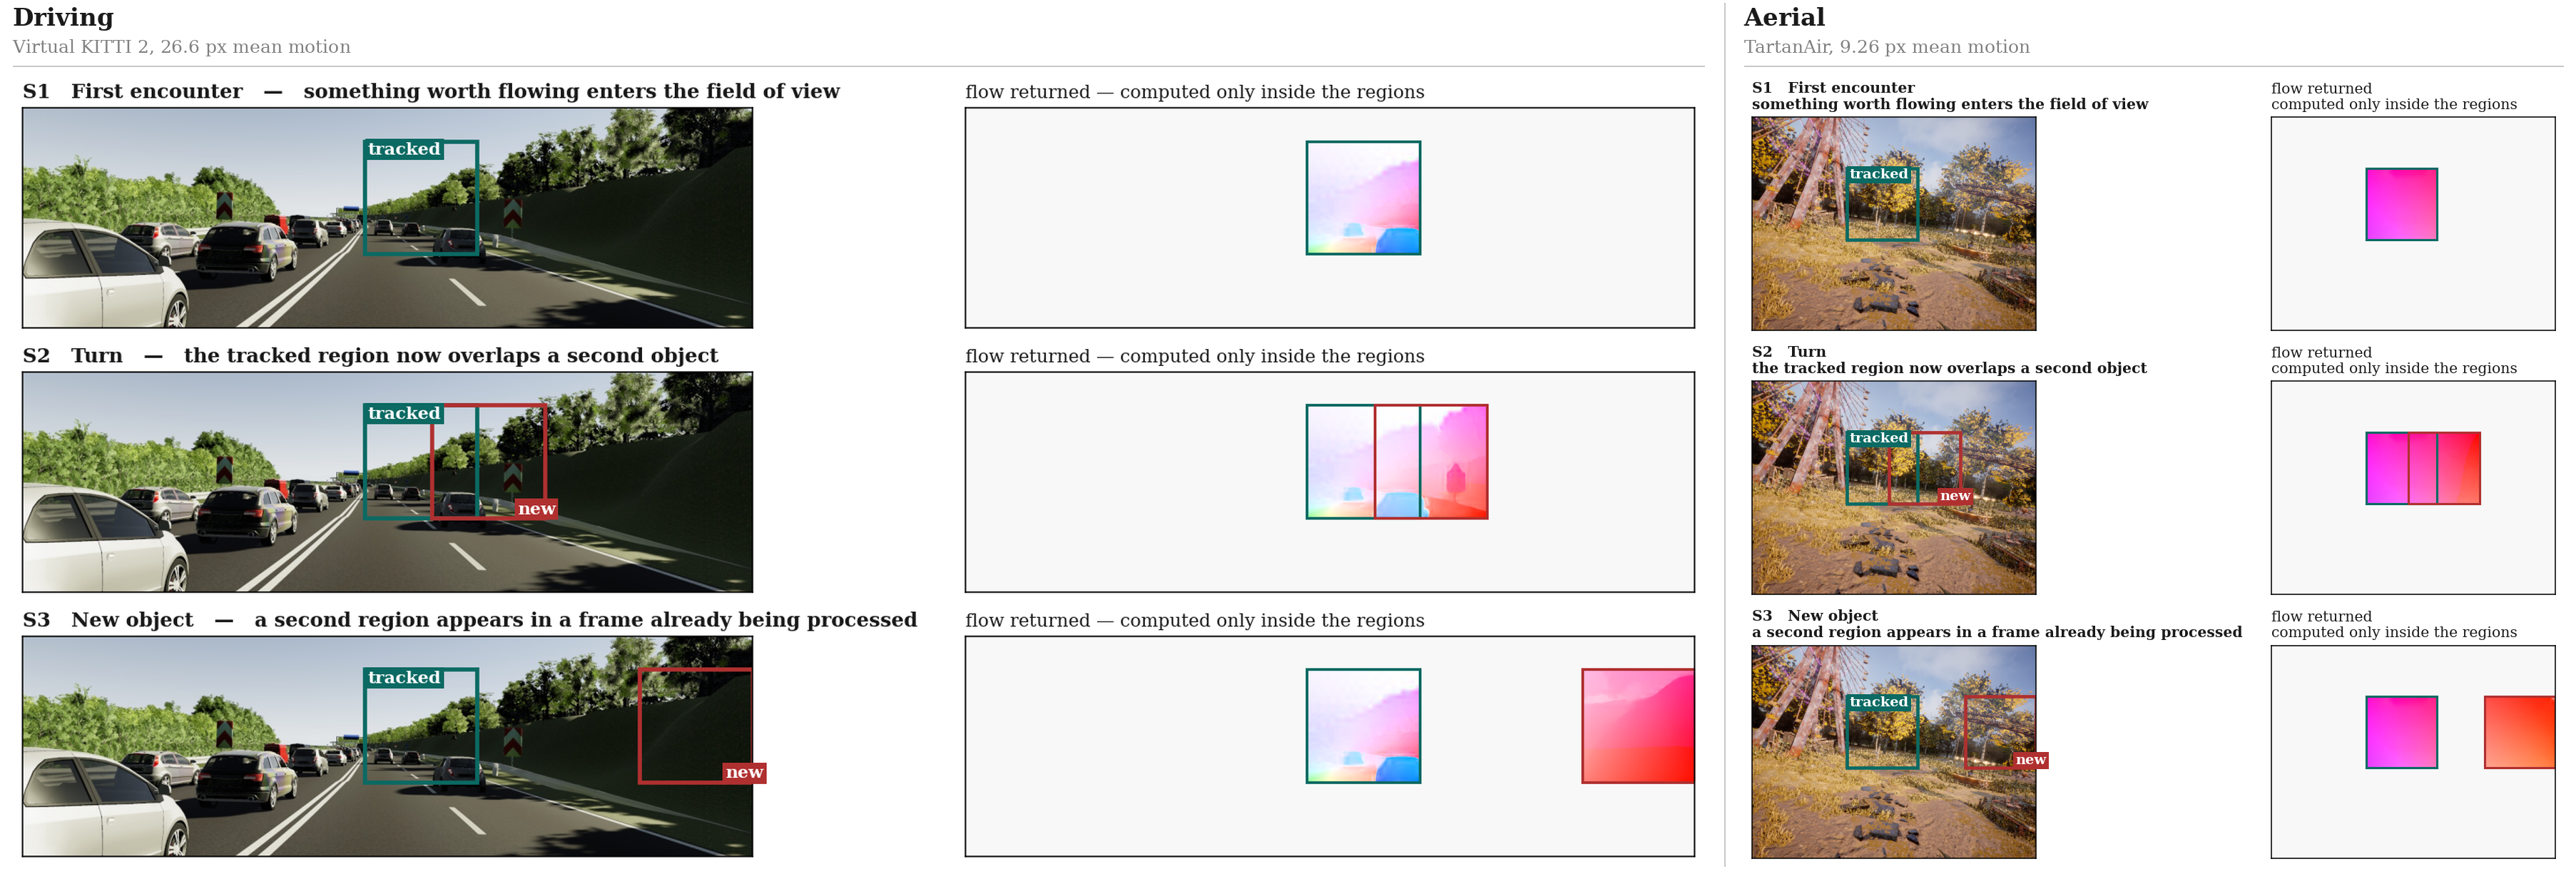
\includegraphics[width=\textwidth]{figures/scenarios_two_domain.png}
\caption{The same three situations in both evaluation domains, with identical
region geometry and decoder configuration; only the domain changes. Left,
driving (Virtual KITTI~2, 26.6\px\ mean inter-frame motion); right, aerial
(TartanAir, 9.26\px). Teal marks the tracked region and red a region that
appears later. Everything outside the marked regions is never computed. Neither
model in this study was trained on aerial imagery.}
\label{fig:twodomain}
\end{figure*}

Region-directed inference is not specific to driving footage.
Fig.~\ref{fig:twodomain} shows the same three situations in both domains under
identical region geometry, which differ by roughly a factor of three in mean
inter-frame motion.

On aerial sequences the decoder is ahead of the baseline at all seven margin
settings tested, by 0.004 to 0.029\px\ (0.777 against 0.781 at full frame). We
note this is the only unconfounded direct comparison in the study: every driving
result is measured on a domain the decoder trained on and the baseline did not,
whereas neither model has seen aerial imagery. The effect is small and measured
on 40 pairs under one seed; it is consistent across seven settings, but the
decoder remains slightly worse on large-motion failures (7.2\% against 6.5\%).

\subsection{Region-Directed Inference}

\begin{table}[t]
\caption{Processing a region instead of the frame, RTX 4060 laptop}
\label{tab:roi}
\centering
\begin{tabular}{lrrr}
\toprule
Region & Latency & Speedup & EPE \\
\midrule
Full frame & 33.3\ms & $1.0\times$ & 0.657 \\
ROI, no margin & 7.8\ms & $4.3\times$ & 1.089 \\
\textbf{ROI +32\px\ margin} & \textbf{7.6\ms} & \textbf{$4.4\times$} & \textbf{0.691} \\
ROI +64\px\ margin & 8.1\ms & $4.1\times$ & 0.667 \\
ROI +128\px\ margin & 9.9\ms & $3.4\times$ & 0.655 \\
\bottomrule
\end{tabular}
\end{table}

\begin{table}[t]
\caption{The region saving is device-dependent; the accuracy cost is not. Same
script, same 40 pairs, $192{\times}192$ region with a 32\px\ margin.}
\label{tab:device}
\centering
\footnotesize
\setlength{\tabcolsep}{4pt}
\begin{tabular}{lrrrr}
\toprule
Device & Full frame & Region & Speedup & EPE cost \\
\midrule
RTX 4060 laptop & 33.3\ms & 7.6\ms & $4.4\times$ & $+0.034$ \\
Tesla V100 & 17.8\ms & 15.1\ms & $1.2\times$ & $+0.034$ \\
\bottomrule
\end{tabular}
\end{table}

A platform that cannot afford full-frame flow must process only the region that
matters. Table~\ref{tab:roi} quantifies this for a $192{\times}192$ region of
interest. Retaining full resolution and processing roughly 14\% of the frame
area costs 0.034\px\ and runs $4.4\times$ faster on the laptop GPU.

The saving, but not the cost, depends on the device (Table~\ref{tab:device}). The
same configuration is $4.4\times$ faster on an RTX 4060 laptop and only
$1.2\times$ faster on a Tesla V100, whose kernel launch overhead dominates at
this region size, so removing 86\% of the pixels removes almost no work. The
accuracy penalty is $+0.034\px$ on both devices to three decimals, since it is
the same computation. We report the two separately rather than averaging them:
the technique pays on constrained hardware, which is the deployment target, and
not on a datacenter GPU.

The context margin is not optional. Without one, error rises by 0.432\px\ and
24\% of large-motion pixels fail outright, because global matching loses the
context it uses to locate distant correspondences. We emphasise that this
technique applies to any flow network including the baseline; it is a property of
the architecture family, not of the queryable decoder.

\subsection{The Margin Rule}

\begin{figure*}[t]
\centering
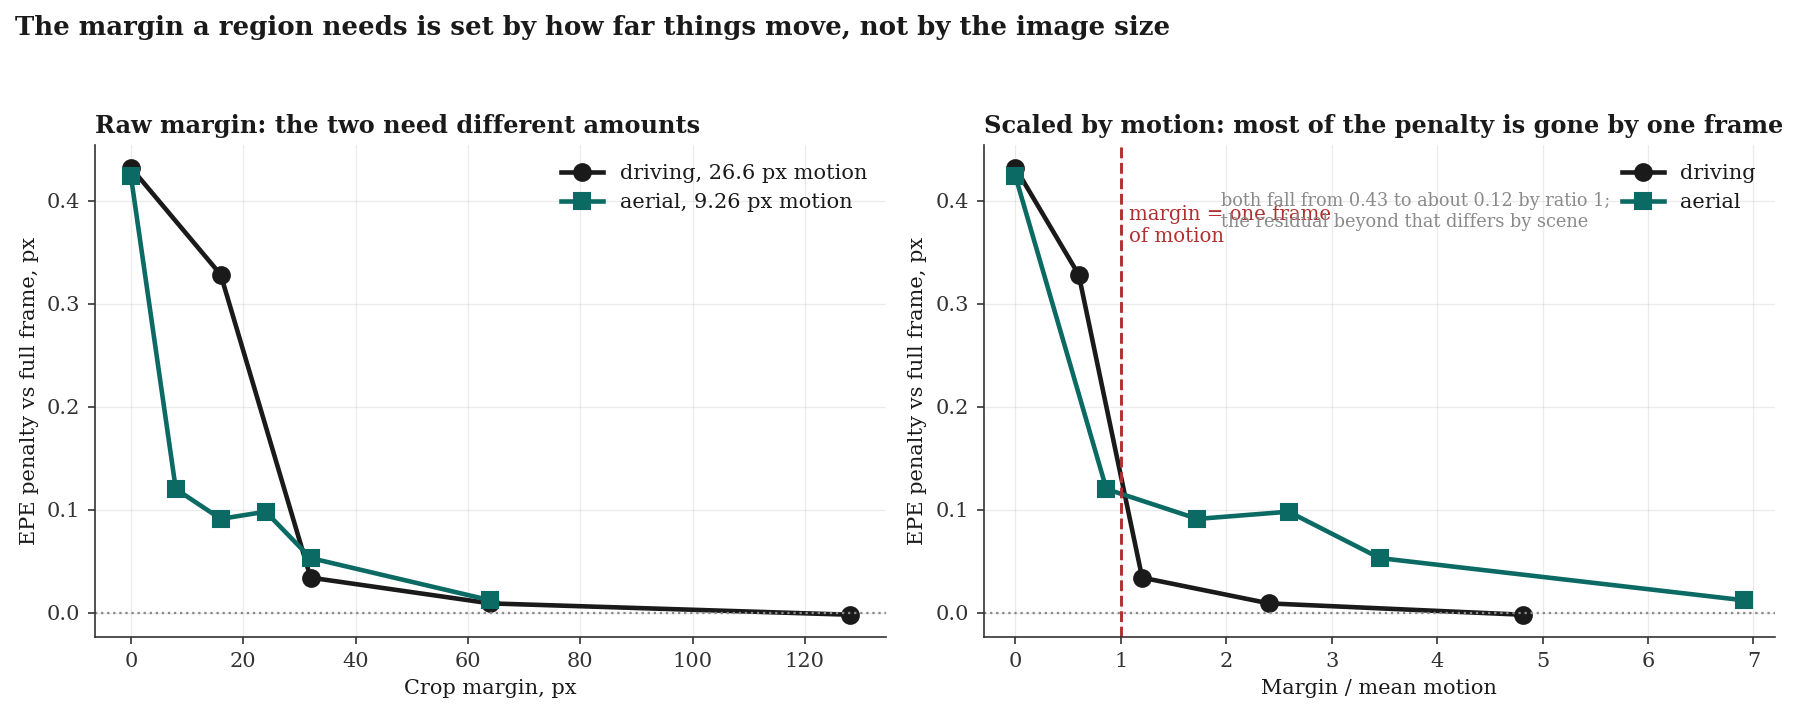
\includegraphics[width=0.92\textwidth]{figures/margin_rule.png}
\caption{Left: in raw pixels the two domains need different margins. Right:
expressed as a multiple of mean inter-frame motion, both shed the bulk of the
penalty by a ratio of one. Measured with the baseline network, since the effect
belongs to the architecture family rather than to the decoder.}
\label{fig:margin}
\end{figure*}

\begin{table}[t]
\caption{EPE penalty in pixels against the full-frame result as a function of
context margin, measured with the baseline network. Mean inter-frame motion is
26.6\px\ for driving and 9.26\px\ for aerial.}
\label{tab:margin}
\centering
\begin{tabular}{rr@{\qquad}rr}
\toprule
\multicolumn{2}{c}{Driving (VKITTI2)} & \multicolumn{2}{c}{Aerial (TartanAir)} \\
\cmidrule(r){1-2} \cmidrule(l){3-4}
Margin & Penalty & Margin & Penalty \\
\midrule
0   & $+0.432$ & 0  & $+0.424$ \\
16  & $+0.328$ & 8  & $+0.120$ \\
32  & $+0.034$ & 16 & $+0.091$ \\
64  & $+0.009$ & 24 & $+0.098$ \\
128 & $-0.002$ & 32 & $+0.053$ \\
    &          & 64 & $+0.012$ \\
\bottomrule
\end{tabular}
\end{table}

If the margin requirement is set by displacement rather than by image size, it
should scale with motion. We test this on aerial sequences whose mean
displacement is a third of the driving case. Both domains begin from
essentially the same penalty with no margin, 0.432 and 0.424\px, and both shed
most of it once the margin reaches approximately one frame of motion
(Table~\ref{tab:margin}, Fig.~\ref{fig:margin}), giving

\begin{equation}
\text{margin} \;\approx\; \text{inter-frame displacement} \;\approx\;
\frac{\text{platform speed}}{\text{frame rate}} .
\end{equation}

This can be evaluated before any flow is computed. The agreement is close up to
that point and the residuals beyond it differ by scene, so the relation predicts
the scale of the required margin rather than the exact curve.

\subsection{Answering an Unanticipated Query}

\begin{table}[t]
\caption{Cost of a new region appearing mid-frame}
\label{tab:s3}
\centering
\begin{tabular}{lrr}
\toprule
Policy & Cost & EPE \\
\midrule
\textbf{v3, sparse queries} & \textbf{1.68\ms} & 2.10 \\
v3, dense region & 4.36\ms & 1.77 \\
v2, new cropped pass & 7.29\ms & 3.60 \\
v3, new cropped pass & 8.23\ms & 3.61 \\
\bottomrule
\end{tabular}
\end{table}

A platform frequently discovers a second region of interest after a frame is
already in flight. This is the case cheap repeatability exists for. Because the
coarse state is cached, the decoder answers for 1.68\ms. A cropped pipeline must
execute an entire new pass, and is markedly less accurate doing so because a
fresh crop has again lost global context (Table~\ref{tab:s3}). Two disjoint crops
cost more than one full frame, giving a simple policy: crop once, or not at all.

\section{Discussion}

The contribution is an operating point rather than a leaderboard position. The
decoder trades 2.6\% of mean accuracy on its training domain for three properties
the fixed-resolution design cannot express, from a model 13.3\% smaller whose
output stage is 38\% of the size of the one it replaces.

For an application that consumes one complete dense field per frame and nothing
else, the baseline remains the correct choice: it is more accurate and 11\%
faster in that mode, 33.3\ms\ against 37.1\ms. The decoder earns its place when
the consumer selects its own query points, revisits a frame, requires positions
between pixels, or needs a confidence value with each correspondence.

We note that the third objective reframes the first two. Mean error over all
pixels is the metric on which the decoder loses, and it is the only operating
point available to a model without confidence. Permitted to abstain, the same
decoder is more than twice as accurate as the baseline over most of the frame.
The architecture costs 0.060\px\ on the mean; the confidence it makes possible
returns 1.27\px\ over 80\% of the frame.

\section{Limitations}

\textbf{Accuracy.} The decoder is less accurate than the upsampler it replaces.
The cause is structural: its finest input is at $1/8$ resolution, so the evidence
available to it varies little within an $8{\times}8$ cell, whereas the baseline's
upsampler reads the full-resolution frame directly. Three independent experiments
converge on this diagnosis. Fourier positional encoding of the sub-cell offset
produced no change, ruling out missing positional signal; querying below the
input sampling rate matched bilinear upsampling exactly; and sub-pixel querying
recovers little beyond interpolation. One mechanism accounts for all three.

\textbf{Sub-pixel querying.} For the same reason, evaluation between input pixels
is presently closer to interpolation than to inference. The interface is exact
and the mechanism is real, but the additional information recoverable between
pixels is small while the decoder's finest input remains at $1/8$ resolution.

\textbf{Embedded validation.} All latency figures are from a laptop GPU. No
measurement on embedded hardware has been performed, so the edge-deployment
premise remains a design target rather than a result. The region speedup is
additionally device-dependent, $4.4\times$ on the RTX 4060 laptop against
$1.2\times$ on a Tesla V100, as reported above.

\textbf{One primary evaluation domain.} Virtual KITTI 2 is synthetic driving
footage, partly answered by 40 aerial pairs from a second domain.

\textbf{Statistical resolution.} One seed per configuration, with
checkpoint-to-checkpoint variation of up to 0.038\px. Differences below
approximately 0.05\px\ are not resolved by this study.

\section{Conclusion}

We replaced the fixed upsampler of a real-time optical flow network with an
implicit decoder answering queries at arbitrary continuous coordinates, and
measured what the substitution costs and provides against three objectives.
Queryable output is affordable: arbitrary continuous coordinates in $O(N)$ rather
than $O(H{\times}W)$, for 2.6\% of mean accuracy, from a model 13.3\% smaller
whose decoder is 38\% of the size of the stage it replaced. Cheap repeatability
is the structural win: a frame pair is processed once and cached, and every query
after the first costs 1.25\ms\ against 33.3\ms, because the baseline keeps no
state between calls. Calibrated confidence is worth more than the mean it costs:
the architecture costs 0.060\px\ on the mean, and abstaining on the least
confident fifth returns 1.27\px\ over the remaining 80\% of the frame.

We additionally characterised region-directed inference for fast platforms,
establishing that a cropped region requires a context margin proportional to
inter-frame displacement, a relation that holds across a threefold difference in
motion scale and can be evaluated from platform speed and frame rate in advance.

Future work is directed by what this study could not settle. Embedded measurement
on Jetson hardware is required before the deployment premise can be claimed, and
nothing else here turns on a laptop GPU the way that claim does. A second seed
per configuration would let the training mixes be ranked honestly, since three of
the four differ by less than the noise floor. Evaluation above the input sampling
rate, against ground truth at twice the input resolution, would test the
arbitrary-resolution capability directly, and it is the one test the baseline
structurally cannot take. Tiled refinement is the largest remaining speed
opportunity, since refinement is 60\% of runtime and all its operations are
local, though it would benefit the baseline equally. Finally, registration on
field and survey imagery would test the intended application and address the
single-domain limitation directly.

\balance

\begin{thebibliography}{99}

\bibitem{neuflow2}
Z.~Zhang, A.~Gupta, H.~Jiang, and H.~Singh, ``NeuFlow v2: High-efficiency optical
flow estimation on edge devices,'' \emph{arXiv:2408.10161}, 2024.

\bibitem{hs81}
B.~K.~P. Horn and B.~G. Schunck, ``Determining optical flow,'' \emph{Artificial
Intelligence}, vol.~17, no.~1--3, pp.~185--203, 1981.

\bibitem{lk81}
B.~D. Lucas and T.~Kanade, ``An iterative image registration technique with an
application to stereo vision,'' in \emph{Proc. Int. Joint Conf. Artificial
Intelligence (IJCAI)}, 1981, pp.~674--679.

\bibitem{brox04}
T.~Brox, A.~Bruhn, N.~Papenberg, and J.~Weickert, ``High accuracy optical flow
estimation based on a theory for warping,'' in \emph{Proc. European Conf.
Computer Vision (ECCV)}, 2004.

\bibitem{flownet}
A.~Dosovitskiy, P.~Fischer, E.~Ilg, P.~H\"{a}usser, C.~Hazirbas, V.~Golkov,
P.~van~der~Smagt, D.~Cremers, and T.~Brox, ``FlowNet: Learning optical flow with
convolutional networks,'' in \emph{Proc. IEEE Int. Conf. Computer Vision (ICCV)},
2015.

\bibitem{flownet2}
E.~Ilg, N.~Mayer, T.~Saikia, M.~Keuper, A.~Dosovitskiy, and T.~Brox, ``FlowNet
2.0: Evolution of optical flow estimation with deep networks,'' in \emph{Proc.
IEEE Conf. Computer Vision and Pattern Recognition (CVPR)}, 2017.

\bibitem{pwcnet}
D.~Sun, X.~Yang, M.-Y. Liu, and J.~Kautz, ``PWC-Net: CNNs for optical flow using
pyramid, warping, and cost volume,'' in \emph{Proc. IEEE Conf. Computer Vision
and Pattern Recognition (CVPR)}, 2018.

\bibitem{liteflownet}
T.-W. Hui, X.~Tang, and C.~C. Loy, ``LiteFlowNet: A lightweight convolutional
neural network for optical flow estimation,'' in \emph{Proc. IEEE Conf. Computer
Vision and Pattern Recognition (CVPR)}, 2018.

\bibitem{raft}
Z.~Teed and J.~Deng, ``RAFT: Recurrent all-pairs field transforms for optical
flow,'' in \emph{Proc. European Conf. Computer Vision (ECCV)}, 2020.

\bibitem{gmflow}
H.~Xu, J.~Zhang, J.~Cai, H.~Rezatofighi, and D.~Tao, ``GMFlow: Learning optical
flow via global matching,'' in \emph{Proc. IEEE/CVF Conf. Computer Vision and
Pattern Recognition (CVPR)}, 2022.

\bibitem{neuflow1}
Z.~Zhang, H.~Jiang, and H.~Singh, ``NeuFlow: Real-time, high-accuracy optical
flow estimation on robots using edge devices,'' \emph{arXiv:2403.10425}, 2024.

\bibitem{nerf}
B.~Mildenhall, P.~P. Srinivasan, M.~Tancik, J.~T. Barron, R.~Ramamoorthi, and
R.~Ng, ``NeRF: Representing scenes as neural radiance fields for view
synthesis,'' in \emph{Proc. European Conf. Computer Vision (ECCV)}, 2020.

\bibitem{siren}
V.~Sitzmann, J.~N.~P. Martel, A.~W. Bergman, D.~B. Lindell, and G.~Wetzstein,
``Implicit neural representations with periodic activation functions,'' in
\emph{Advances in Neural Information Processing Systems (NeurIPS)}, 2020.

\bibitem{liif}
Y.~Chen, S.~Liu, and X.~Wang, ``Learning continuous image representation with
local implicit image function,'' in \emph{Proc. IEEE/CVF Conf. Computer Vision
and Pattern Recognition (CVPR)}, 2021.

\bibitem{anyflow}
H.~Jung, Z.~Hui, L.~Luo, H.~Yang, F.~Liu, S.~Yoo, R.~Ranjan, and D.~Demandolx,
``AnyFlow: Arbitrary scale optical flow with implicit neural representation,'' in
\emph{Proc. IEEE/CVF Conf. Computer Vision and Pattern Recognition (CVPR)}, 2023.

\bibitem{infinidepth}
H.~Yu, H.~Lin, J.~Wang, J.~Li, Y.~Wang, X.~Zhang, Y.~Wang, X.~Zhou, R.~Hu, and
S.~Peng, ``InfiniDepth: Arbitrary-resolution and fine-grained depth estimation
with neural implicit fields,'' in \emph{Proc. IEEE/CVF Conf. Computer Vision and
Pattern Recognition (CVPR)}, 2026. arXiv:2601.03252.

\bibitem{kendall}
A.~Kendall and Y.~Gal, ``What uncertainties do we need in Bayesian deep learning
for computer vision?'' in \emph{Advances in Neural Information Processing Systems
(NeurIPS)}, 2017.

\bibitem{ilg18}
E.~Ilg, O.~Cicek, S.~Galesso, A.~Klein, O.~Makansi, F.~Hutter, and T.~Brox,
``Uncertainty estimates and multi-hypotheses networks for optical flow,'' in
\emph{Proc. European Conf. Computer Vision (ECCV)}, 2018.

\bibitem{pdcnet}
P.~Truong, M.~Danelljan, L.~Van~Gool, and R.~Timofte, ``Learning accurate dense
correspondences and when to trust them,'' in \emph{Proc. IEEE/CVF Conf. Computer
Vision and Pattern Recognition (CVPR)}, 2021.

\bibitem{vkitti2}
Y.~Cabon, N.~Murray, and M.~Humenberger, ``Virtual KITTI 2,''
\emph{arXiv:2001.10773}, 2020.

\bibitem{tartanair}
W.~Wang, D.~Zhu, X.~Wang, Y.~Hu, Y.~Qiu, C.~Wang, Y.~Hu, A.~Kapoor, and
S.~Scherer, ``TartanAir: A dataset to push the limits of visual SLAM,'' in
\emph{Proc. IEEE/RSJ Int. Conf. Intelligent Robots and Systems (IROS)}, 2020.

\end{thebibliography}

\end{document}
